% !TEX root = ../main.tex
% =====================================================================
% 5. RESULTS
%
% Rules for this section:
%   - the tables carry the results; the prose says only what to notice
%   - no number appears twice
%   - readable model names (encoder + pooling head); configuration
%     identifiers stay in the appendix leaderboard
% Every number comes from the stored results files.
% =====================================================================

\section{Results}
\label{sec:results}

Seventy-two model variants were compared: the \seanet{} encoders paired with the proposed pooling
heads and with \millet{}'s heads, plus the FCN, ResNet and InceptionTime baselines re-trained here,
each run on \webtraffic{} and on the \ucr{} archive -- up to 129 datasets per model. Two conventions
hold throughout: starred rows were trained with 3 seeds and report the mean, every other row is a
single seed (\Cref{sec:setup:protocol}); and a number produced here never shares a column with a
number copied from \citet{early2024millet}, because the two use different training configurations.

% ---------------------------------------------------------------------
\subsection{Main comparison on \webtraffic{}}
\label{sec:res:web}

\webtraffic{} is the only dataset on which classification quality and explanation correctness can
both be measured (\Cref{sec:setup:data}), which makes \Cref{tab:web_main} the principal table of
this report.

\begin{table}[tbp]
\caption{The ten best models on \webtraffic{}, ranked by accuracy, with the re-trained baselines
below. Every model is written as \emph{encoder $+$ pooling head}; the corresponding configuration
identifiers, and the other 62 models, are in the full leaderboard published with the code
(\Cref{sec:setup:baselines}). Starred rows were trained with
3 seeds and show the mean, with the per-seed values in \Cref{tab:seeds}; all other rows are a single
seed. Higher is better for accuracy, AOPCR and NDCG@$n$, lower for parameters. AOPCR is not
normalised (\Cref{sec:bg:metrics}), so it compares rows of this table with each other and never with
a value printed in another paper.}
\label{tab:web_main}
\begin{center}
\footnotesize
\setlength{\tabcolsep}{3.2pt}
\begin{tabular}{rlcccr}
\toprule
\textbf{\#} & \textbf{Model (encoder $+$ pooling head)} & \textbf{Accuracy} & \textbf{AOPCR} &
\textbf{NDCG@$n$} & \textbf{Params} \\
\midrule
1  & \seanet{} gated (mean) $+$ Top-$k$$^\ast$        & \textbf{0.955} & 2.225 & 0.750 & 61{,}740 \\
2  & \seanet{} base $+$ conjunctive \reused           & 0.954 & 1.502 & 0.698 & 269{,}083 \\
3  & \seanet{} gated (max) $+$ Top-$k$                & 0.952 & 2.268 & 0.719 & 61{,}740 \\
4  & \seanet{} spike/trend $+$ Top-$k$                & 0.950 & 2.316 & 0.756 & 67{,}020 \\
5  & \seanet{} multi-scale channels (input-gated base) $+$ Top-$k$ & 0.948 & 2.316 & 0.757 & 69{,}768 \\
6  & \seanet{} multi-scale channels (gated base) $+$ Top-$k$ & 0.948 & 2.223 & 0.717 & 67{,}592 \\
7  & \seanet{} bottleneck $+$ Top-$k$$^\ast$          & 0.947 & 2.621 & \textbf{0.773} & \textbf{41{,}324} \\
8  & \seanet{} reconstruction-residual $+$ adaptive class-wise & 0.946 & 2.601 & 0.768 & 62{,}935 \\
9  & \seanet{} input-gated $+$ Top-$k$                & 0.946 & \textbf{2.803} & 0.748 & 58{,}092 \\
10 & \seanet{} base $+$ class-wise conjunctive        & 0.946 & 1.722 & 0.686 & 269{,}164 \\
\midrule
\multicolumn{6}{l}{\emph{Also discussed in this report}}\\
   & \seanet{} input-gated $+$ adaptive class-wise$^\ast$ & $0.905\pm0.030$ & $2.651\pm0.437$ & 0.732 & 58{,}102 \\
\midrule
\multicolumn{6}{l}{\emph{Baselines re-trained here, identical training configuration}}\\
   & \millet{} (InceptionTime $+$ conjunctive)$^\ast$ & $0.887\pm0.010$ & $2.569\pm0.884$ & 0.677 & 423{,}707 \\
   & ResNet $+$ conjunctive                           & 0.772 & 2.952 & 0.554 & 506{,}331 \\
   & FCN $+$ conjunctive                              & 0.742 & 3.826 & 0.533 & 267{,}035 \\
\bottomrule
\end{tabular}
\end{center}
\end{table}
% Source: results/SEA_NET/leaderboard.csv, ranks 1-11 by web_acc, with rank 4 (seanet_topk_nofocus)
% dropped because it is not a separate model -- it is the ablation of rank 8 with the focus penalty
% switched off, and it is reported as such in Appendix B. Row 5 = seanet_inputgate_mschan,
% row 6 = seanet_gated_mschan (both use the sea_multiscale_channels wrapper, over a different base).
% Starred rows: the seed-averaged web_acc / web_aopcr / web_ndcg columns, which equal the mean over
% the WebTraffic rows of each model's results.csv (seeds 0/1/2).
% NOTE: leaderboard.csv's millet_acc (0.8445) is the published UCR-85 mean, NOT a WebTraffic number.

Four observations follow from \Cref{tab:web_main}. First, all ten leading models are \seanet{}
models, and each of them exceeds the best re-trained baseline (0.887). Second, the top ten span only
nine thousandths of accuracy, from 0.946 to 0.955, which is why \Cref{sec:disc:reading} declines to
name a winner on accuracy alone. Third, the parameter column separates models that the accuracy
column does not: ranks 2 and 10 require about 269\,K parameters to reach the accuracy that rank 7
attains with 41\,K. Fourth, and this is the central result, \mbot{} (rank 7) has both the best
NDCG@$n$ of the table (0.773) and the smallest parameter count, so no classification or explanation
quality was traded for the reduction in size. This is what Top-$k$ pooling was designed to achieve
(\Cref{sec:pool:topk}): by averaging only the $k$ most decisive time steps, the interpretation is
exactly zero wherever the model used no evidence, whereas the baseline's importance curve never
quite reaches zero and its extent has to be guessed (\Cref{fig:teaser}).

The reduction holds on the quantities a device constrains. Measured on the real \webtraffic{} input,
\mbot{} uses 90\,\% fewer parameters than the re-trained \millet{} baseline, its saved file shrinks
from 4.11\,MB to 1.43\,MB, and one prediction is about 1.6 times faster; the file size is what matters
for the microcontroller target. \Cref{tab:cost} gives the full cost comparison, including its
counterpart: the \seanet{} models take two to three times \emph{longer to train}.
\Cref{fig:web_bars} places quality and cost side by side for the five most accurate models.

\begin{figure}[tbp]
  \centering
  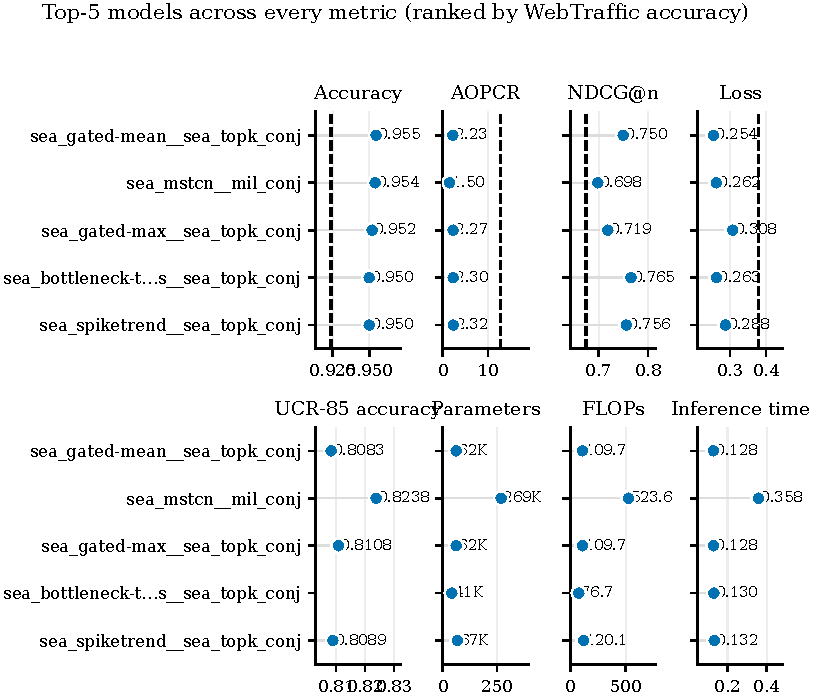
\includegraphics[width=0.78\linewidth]{results/paper_figures/01_main_figures/topk5_multimetric}
  \caption{The five most accurate models on \webtraffic{} across every metric measured -- all five
  are \seanet{} models. One row is one model and the row order is identical in every panel, so a
  model can be followed from the quality panels (accuracy, AOPCR, NDCG@$n$, loss) to the cost panels
  (\ucr{}-85 accuracy, parameters, compute, prediction time). The contrast between the two blocks is
  the point: the models at the top of the quality panels sit at the inexpensive end of the cost
  panels. The clearest case is the second row on accuracy, the \seanet{} base encoder with
  \millet{}'s conjunctive head, which needs roughly six times the parameters of \mbot{} while being
  five thousandths more accurate.}
  \label{fig:web_bars}
\end{figure}

% ---------------------------------------------------------------------
\subsection{Accuracy across the 85 \ucr{} datasets}
\label{sec:res:ucr}

A single dataset cannot support a general claim, so the same models were evaluated on the 85 \ucr{}
datasets for which \millet{} results are published. \Cref{tab:ucr_accuracy} reports the mean accuracy
with the mean rank and the per-dataset record beside it, because a mean alone can be dominated by a
few datasets (\Cref{sec:setup:protocol}).

\begin{table}[tbp]
\caption{Accuracy over the \ucr{} datasets published by \millet{}. ``Mean rank'' is the average
accuracy rank over the 84 datasets shared by the 28 models evaluated on the complete archive
(lower is better). ``W/T/L'' is the win / tie / loss record per dataset against the \emph{published}
\millet{} numbers, a tie meaning the two accuracies are within 0.005. The two \millet{} rows differ
only in the training configuration; the architecture and the code are identical.}
\label{tab:ucr_accuracy}
\begin{center}
\footnotesize
\begin{tabular}{lccc}
\toprule
\textbf{Model} & \textbf{Mean accuracy} & \textbf{Mean rank} &
\textbf{W/T/L vs published} \\
\midrule
\mgat{}                      & 0.8083 & 15.29 & 18 / 13 / 53 \\
\mbot{}                      & 0.8097 & 15.40 & 19 / 15 / 50 \\
\minp{}                      & 0.8153 & 15.47 & 19 / 15 / 50 \\
ResNet $+$ conjunctive       & 0.8146 & 13.54 & 25 / 11 / 48 \\
FCN $+$ conjunctive          & 0.8141 & 14.48 & 20 / 12 / 52 \\
\midrule
\millet{}, re-trained (configuration of \Cref{tab:protocol}) & 0.8274 & 12.60 & 13 / 25 / 46 \\
\millet{}, re-trained (\emph{their} own configuration) & \textbf{0.8434} & \textbf{9.41} &
                                                  \textbf{26 / 32 / 26} \\
\midrule
\millet{} \citep{early2024millet}, published & 0.8445 & -- & -- \\
\bottomrule
\end{tabular}
\end{center}
\end{table}
% Mean accuracy: leaderboard.csv, ucr85_acc column (averaged over the datasets each model finished
% and over every seed it has). Mean rank + W/T/L: results/paper_figures/tables/table_ranking_accuracy.csv,
% regenerated 2026-08-12 after millet_paper finished -- computed over the 84 datasets every
% fully-swept model shares.
% millet_paper (their recipe): ucr85_n = 84, ucr85_acc = 0.8434, rank 9.41, W/T/L 26/32/26.
% millet     (my recipe):      ucr85_n = 84, ucr85_acc = 0.8274, rank 12.60, W/T/L 13/25/46.
% The published row: millet_acc = 0.8445 from leaderboard.csv. Mean rank and W/T/L are left blank
% because the published per-dataset numbers needed to compute them were never carried through.

This table tells a different story from \Cref{tab:web_main}. Over the \ucr{} archive both \millet{}
rows are ahead of all three \seanet{} models, which lose more datasets than they win. This does not
invalidate the \webtraffic{} result but it bounds it: both headline models were selected because they
performed well on \webtraffic{} (\Cref{sec:setup:data}), and one dataset does not predict behaviour
on 85 heterogeneous ones. \seanet{} remains competitive -- within one to two accuracy points of the
baseline at about a tenth of the parameters -- but the results do not support a claim of general
superiority.

The last two rows close objective~O2, and they are the \emph{same architecture and the same code}
trained twice under two configurations. Under \Cref{tab:protocol} the model reaches 0.8274; under
\millet{}'s own published configuration it reaches 0.8434 against a published 0.8445, a difference of
about one thousandth, with a balanced record of 26 wins, 32 ties and 26 losses. The earlier shortfall
was therefore a difference in training budget, not a defect in the re-implementation. This also
determines how the rest of the table is read: the \seanet{} models were trained under
\Cref{tab:protocol}, so their correct point of comparison is the 0.8274 row rather than the published
one.

Finally, neither component alone accounts for the result. Averaged over every partner, the encoder
choice moves \webtraffic{} accuracy over a range of 0.858--0.937 and the pooling head choice over
0.744--0.921, two spreads of comparable size, and the best pair is not composed of the two
individually best halves (\Cref{app:ablations}).
